\documentclass{report}
\usepackage[english]{babel}
\usepackage[utf8]{inputenc}
\usepackage[T1]{fontenc}
\usepackage{listings}
\usepackage{titlesec}
\usepackage{color}
\usepackage{graphicx}
\usepackage{geometry}
\geometry{hmargin=2.5cm,vmargin=3.5cm}


\titleformat{\chapter}[display]
            {\normalfont\bfseries}{}{0pt}{\Huge}

\lstset{ escapeinside={(*}{*)} }

\title{\textbf{Rapport IA PROG6}\\Pingouin}

\author{Castel Antonin, Reboul Paul, Soret Louka, Sorin Gaëtan, Vandendorpe Thomas}
\begin{document}

\maketitle{}
\tableofcontents
\chapter{Introduction}
Le jeu Pingouin est un jeu à somme nulle où un certain nombre de joueurs s'affrontent à tour de rôles. Une IA difficile peut donc utiliser un algorithme de type MinMax pour évaluer les coups possibles.Pour créer l'IA la plus efficace possible, nous avons identifié quatre grandes phases de jeu lors du déroulement de chaque parties :

-Le placement des pingouins en début de partie sur les cases à un poisson.

-Les déplacements en début de partie, lorsque l'algorithme MinMax ne calcule pas assez de coups à l'avance pour différencier avec pertinence les différents coups possibles.

-Après plusieurs coups, où les coups d'avance que calcule le MinMax sont 
suffisants pour évaluer la qualité d'un coup.

-La fin de partie, où les pingouins sont seuls sur des îles et qu'il faut faire le parcours le plus avantageux.
Nous allons donc détailler ici comment son gérées ces différentes phases dans notre IA difficile, et comment sont utilisés des parties de l'IA difficile pour créer des IA plus simples.
\chapter{IA Difficile}
Notre IA difficile à une stratégie bien définie, à la fois maximiser le nombre de poissons récupérés et faire des îles, soit pour enfermer les pingouins ennemis, soit pour s'assurer une grande quantité de poissons en fin de parti\setlength{\topmargin}{0cm}
e.
Pour ce faire, nous avons utilisé un algorithme de type MinMax avec élagage Alpha-Beta.
\section{Placement en debut de partie}
En début de partie, il n'est possible de se placer que sur des cases contenant un seul poisson, nous calculons donc une valeur heuristique sur toutes les cases contenant un seul poisson, et notre pingouin est placé sur la case ayant la valeur la plus élevée.
Ces valeurs sont calculées en fonction du nombre de cases a trois poissons voisines accessibles. 
\newline
On prend aussi en compte que placer un pingouin sur un bord de la carte n'est pas une bonne idée (encore moins dans un coin), ainsi que du fait qu'il faut éviter de mettre tout ses pingouins dans la même zone de la carte.
\newline
On prend aussi en compte le placement des pingouins ennemis, car on tente de les priver du plus grand nombre de cases possible.


\section{Heuristique}
Nous évaluons les feuilles de l'arbre, donc nous évaluons le résultat de l'exécution d'un certain nombre de coups sur le plateau initial.
\newline

\vspace{0.3cm}
\textbf{Valeurs calculées sur les feuilles :}
\newline
Les heuristiques sur les feuilles sont calculés en fonction des îles présentes sur le plateau de jeu, et sur les scores des différents joueurs.
\newline
On calcule la liste des îles, et on évalue chacune d'entre elles en fonction du nombre de poissons qu'elle contient ainsi que du nombre de pingouins alliés et ennemis qu'elle contient.
\newline
Par exemple, laisser une île à l'ennemi n'est pas une bonne idée, sauf si tout les pingouins ennemis sont sur cette île et que cette dernière n'a pas suffisamment de poissons pour que l'ennemi puisse gagner.
\newline 
La configuration est donc évaluée en fonction de ses îles et de ce qu'elles contiennent.
\newline 
En particulier,
\newline
-Ne pas laisser de trop grandes parties de banquise à un pingouin ennemi seul.
\newline
-S'isoler sur une grande partie de banquise. 
\newline
-Si possible, isoler des pingouins ennemis sur un seul bout de banquise.
\newline
-Ne pas se faire isoler un pingouin sur un bout de banquise.
\newline
-On évite de laisser des grandes îles sans aucun pingouins dessus. 
\newline
-Si la partie est finie et que notre score est le plus élevé, on renvoie une heuristique maximale.
\newline
-Si un ou plusieurs pingouins ennemis sont isolés sur une île suffisamment grande pour s'assurer la victoire, on renvoie une heuristique minimale.
\newline
\newline
Lorsque deux fils de la racine ont deux valeurs heuristiques identiques, et que cette heuristique est la plus grande, les fils sont départagés en fonction du coup qu'il représentent, dans le but de choisir le coup le plus avantageux directement. 
\vspace{0.3cm}

\section{Fin de partie}
Durant toute la durée de la partie, un pingouin isolé sur son île n'est pas considéré par le MinMax, et ne sera donc jamais déplacé.
C'est donc à la fin de la partie que l'on doit calculer le meilleur chemin sur une île, pour chaque pingouin.
\newline 
Pour ce faire, on calcule un parcours Hamiltonien sur l'île. La complexité pour trouver un parcours Hamiltonien est telle que malheureusement sur une grande île, on ne peut pas le calculer. Quand c'est le cas, on fait un coup qui tente de ne pas briser le parcours Hamiltonien sans le calculer.

\chapter{IA facile et IA moyenne}
\section{IA facile}
L'IA facile se comporte comme l'IA difficile pour la première phase de jeu, mais sa stratégie est très différente, elle n'est pas aléatoire mais essaie de récupérer le plus de poissons possibles en un minimum de coups, elle récupère donc rapidement beaucoup de points, mais elle ne priorise pas forcement le fait de bloquer un ennemi.
Cela donne une IA qui n'est pas très performante quand il y a peu de pingouins pour beaucoup de cases, mais une IA très correcte lorsque la tendance s'inverse.
\newline
L'IA facile ne calcule pas de parcours Hamiltonien lorsqu'un pingouin est seul sur une île, et les pingouins seuls sur des îles peuvent être  déplacés. 

\section{IA moyenne}
L'IA moyenne est basée sur l'IA difficile, sauf qu'elle calcule une partie de l'arbre inférieure à l'IA difficile, et par conséquent elle anticipe moins et ses coups sont parfois moins bons.
Dans cette IA, les pingouins seuls sur des îles ne sont déplacés, et en fin de partie on tente de maximiser le nombre de poissons récupérés sur les îles.


\chapter{Changements possibles}
\section{Améliorations possibles des IA}

-L'IA difficile ne change pas de stratégie quand la sienne n'est pas la bonne. Il a été dit auparavant que la stratégie de l'IA facile était très correcte quand le nombre de pingouins est très grand comparé au nombre de cases, par conséquent, l'IA difficile pourrait changer de stratégie dans ce genre de cas.
\newline
-Le parcours Hamiltonien en fin de partie sur les grandes îles est améliorable.
\newline 
-Multi-Threader le calcul de l'arbre pour améliorer significativement la profondeur calculable de ce dernier, et donc largement améliorer le niveau de jeu de l'IA.

\section{Pistes explorées mais non concluantes}
-Utiliser le MinMax pour calculer le parcours Hamiltonien en fin de partie, comme il essaie de maximiser le score, on obtiendrait un chemin correct.
\newline
-Nous avons essayé de modifier la profondeur de calcul de l'arbre localement, pour que les branches prometteuses soit calculées plus profondément que les branches où les premiers coups sont mauvais, mais les résultats n’étaient pas très concluants en terme de niveau de jeu de l'IA.

\chapter{Résultats}
\section{Graphiques}
\begin{center}
  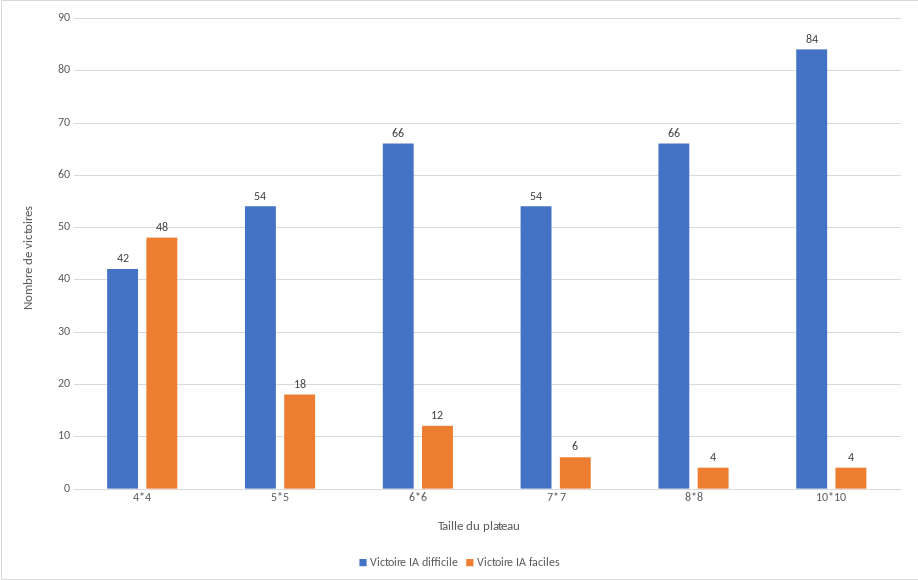
\includegraphics[width=11.5cm]{graph1.png}
  \newline
\textbf{\textit{Facile(bleu) vs Difficile(Rouge) sur différents plateaux.}}
  \newline
  
  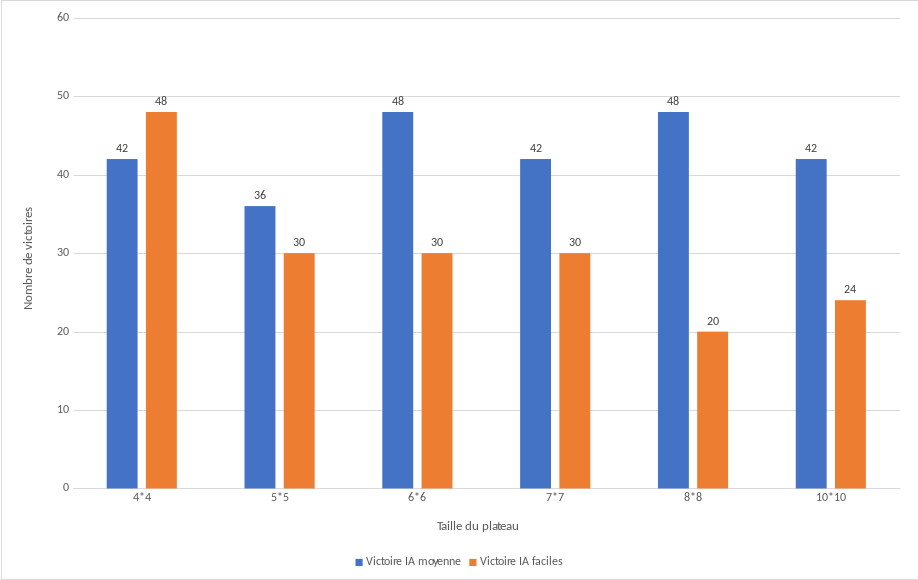
\includegraphics[width=11.5cm]{graph2.png}
  \newline
\textbf{\textit{Facile(Bleu) vs Moyenne(Rouge) sur différents plateaux.}}
  \includegraphics[width=18cm]{graph3.png}
  \newline
\textbf{\textit{Humain(Bleu) vs Difficile(Rouge)}}
\end{center}


\section{Interpretation}

Nous pouvons voir que les IA respectent assez bien la hiérarchie difficile > moyenne > facile entre elles. 
Les parties représentées dans ces graphiques représentent des parties à deux joueurs avec 4 pingouins, les tendances sont exactement les mêmes si on modifie le nombre de pingouins par joueurs.
Cette hiérarchie est aussi assez bien respectée lors des parties avec un nombre de joueurs supérieur à deux, mais vu que nous nous sommes concentrés en priorité sur les parties à deux joueurs, il existe des anomalies que nous n'avons pas eu le temps de résoudre.
\newline
Par exemple, une partie à quatre joueurs, avec 3 IA difficiles et une IA facile sur un plateau de taille standard sera souvent remportée par l'IA facile, simplement car sa stratégie est bien supérieure à celles des IA difficiles dans cette situation.
\newline
Pour ce qui est des tests contre des humains, nous avons choisit différents profils; des gens qui n'avait jamais joué au jeu auparavant, et des joueurs expérimentés.
Les résultats sont assez différents en fonction du type de joueur, les joueurs expérimentés gagnent en général contre l'IA difficile, mais ce sont tout de mêmes des parties assez serrées.
Les joueurs débutant quant à eux, perdent une grande majorité du temps.


\end{document}